





%%%%%%%%%%%%%%%%%%%%%%%%%%%%%%%%%%%%%%%%%%%%%%%%%%%%%%%%%%%%%%%%%%%%%%%%%%%%%%%%%%%%%%%%%%%%%%%%%%%%%%%%%%%%%%%%%%%%%%%%%%%%%%%%%%%%%%%%%%%%%%%%%%%%%
%\begin{frame}[t,fragile]{}
%\begin{block}{}
%	\textcolor{Azul}{Funciones contractivas no uniformemente continuas}  
%\end{block}
 %\textbf{Teoremas del Punto Fijo "tipo Banach"}
%\begin{itemize}
%	\item[$ - $] 1968 Kannan\\
%	\textbf{Definición:}  \\
%	\begin{exampleblock}{}
%		Sean $(X,d)$ un espacio métrico, $\alpha \in (0, \frac{1}{2})$ y $f: X \longrightarrow X$. Se dice que $f$ es $\alpha$-contractiva en el sentido de Kannan, si
%		$$d(f(x), f(y)) \leq \alpha [d(x, f(x)) + d(y, f(y))], \forall x, \ y \in X.$$
%		%A $\alpha$ se le llama constante de contracción de Kannan.
%	\end{exampleblock}
%	\item[$ - $] Una forma de trabajo en espacios métricos. 
%	\item[$ - $] 1973 Hardy-Rogers\\
	
%\end{itemize}

%\end{frame}

%	\begin{frame}[t,fragile]{}
%\begin{block}{}
%	\textcolor{Azul}{¿Cómo generar tipos de funciones contractivas en espacios métricos?} 
%	\end{block}

%\begin{wrapfigure}{r}{-2.5\textwidth}
 %   \centering
  %  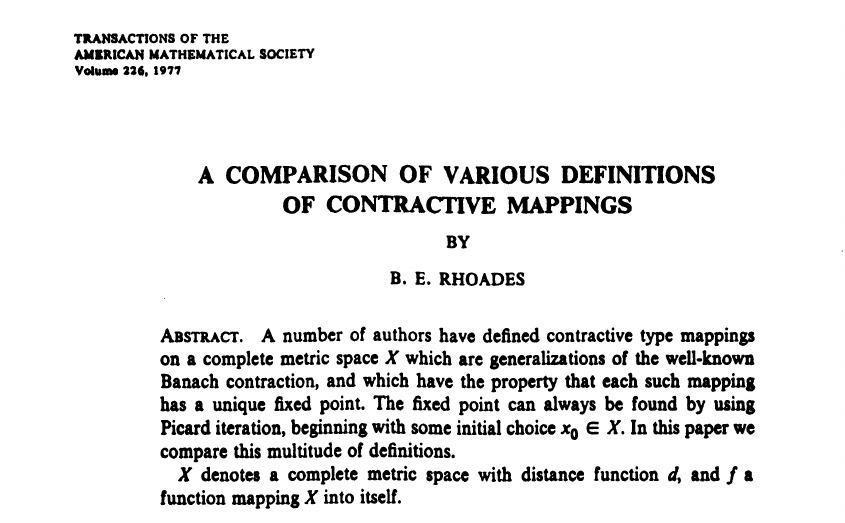
\includegraphics[width=0.6\textwidth]{articulo.jpeg}
    
%\end{wrapfigure}
%Combinaciones de

%\begin{itemize}
 %   \item \ul{$d(x,y)$}
  %  \item \ul{$d(x,T(x))  $}\\
   % \item \ul{$d(x, T(y))  $}\\
    %\item \ul{$ d(y,T(x)) $}\\
%     \item \ul{$ d(y,T(y))  $}
%\end{itemize}
%\end{frame}





 %%%%%%%%%%%%%%%%%%%%%%%%%%%%%%%%%%%%%%%%%%%%%%%%%%%%%%%%%%%%%%%%%%%%%%%%%%%%%%%%%%%%%%%%%%%%%%%%%%%%%%%%%%%%%%%%%%%%%%%%%%%%%%%%%%%%%%%%%%%%%%%%%%%%%
